%\documentclass[10pt, frame]{beamer}
\documentclass[10pt, notes=only]{beamer}
%\documentclass[10pt, notes]{beamer}
\usepackage[utf8]{inputenc}
\usepackage[T1]{fontenc}
\usepackage{lmodern}
\usepackage{microtype}
\usepackage[]{amsmath}
\usepackage{amssymb}
\usepackage{amsfonts}
\usepackage{appendixnumberbeamer}
\usepackage[czech]{babel}
\usepackage[]{hyperref}
\usepackage{booktabs}
\usepackage[]{graphicx}
\usepackage{siunitx}
\usepackage[figurename=]{caption}
%\newcommand{\obr}[1]{Obr. převzat z \cite[#1]}
\usepackage[
    backend=biber
    ,style=iso-numeric
    ,autolang=other
    ,pagetotal=true
    ,sortlocale=cs_CZ
    ,bibencoding=UTF8
    ,spacecolon=false
    ,block=space
]{biblatex}
\addbibresource{citace.bib}

\usetheme[sectionpage=none, numbering=fraction, progressbar=none, block=fill]{metropolis}
\setbeamerfont{note page}{size=\footnotesize}
\author{Michal Šesták}
\title{Infrazvuk}
\subtitle{FNEI}
\institute{}
%\institute{Fakulta jaderná a fyzikálně inženýrská, ČVUT v Praze\\[0.5em]
%Vedoucí práce: Ing. Iva Ambrožová, Ph. D.}
\date{5. 12. 2018}
\begin{document}

\renewcommand{\figurename}{Obr.}
\renewcommand{\tablename}{Tab.}

\maketitle

%\begin{frame}{Obsah}
    %\tableofcontents
%\end{frame}

\begin{frame}
    \begin{itemize}
        \item $\SI{3,21}{mHz}\ (\SI{15}{\celsius})<f< \text{cca}\ \SI{20}{Hz}$ 
        \item $v=\text{cca}\ \SI{340}{m/s}$ u mořské hladiny
        \item \textbf{Zdroje} zemětřesení, dopadající meteority, sopky, vodopády, velké vlny, počasí, zvířata, jaderné exploze, vibrující trubky \dots
        \item \textbf{Vnímání člověkem} tlak v uších i jinde (záleží na intenzitě zvuku), bolesti hlavy, nevolnosti, noční děsy, poruchy spánku, závratě 
        \item \textbf{Využití} monitorování přírodních katastrof; lokalizování ropy a plynu; předpovídání počasí; studium srdce (Balistokardiografie)
        \item \textbf{Kde se je nevyplatí používat} sonar
    \end{itemize}
\end{frame}

\note[itemize]{
\item \textbf{Co to je} Infrasonics, vibrational or stress waves in elastic media, having a frequency below those of sound waves that can be detected by the human ear—i.e., below 20 hertz. The range of frequencies extends down to geologic vibrations that complete one cycle in 100 seconds or longer.
\item \emph{Infrasound is characterized by an ability to cover long distances and get around obstacles with little dissipation.}
\item \textbf{Zvířata} “Elephants, in particular, produce infrasound waves that travel through solid ground and are sensed by other herds using their feet, although they may be separated by hundreds of kilometres.”
\item Zvířata dokážou rozeznat blížící se přírodní katastrofu
\item \textbf{duchové} If infrasound hits at just the right strength and frequency, it can resonate with human eyes, causing them to vibrate. This can lead to distorted vision and the possibility of “ghost” sightings. Or, at least, what some would call ghost sightings. Infrasound may also cause a person to “feel” that there’s an entity in the room with him or her, accompanied by that aforementioned sense of dread.
}
\note[itemize]{
\item \textbf{ropa atd.} Distinctive rock formations in which these minerals are likely to be found can be identified by sonic ranging, primarily at infrasonic frequencies. With an array of seismic detectors, a computational form of holography may be achieved.
\item \textbf{Balistokardiografie} je neinvazivní metoda pro měření ``balistických'' sil srdce, síly srdce pumpovat krev; studuje pohyby těla vznikajících z ejektování krve ze srdce do velkých tepen; normální frekvence pohybů srdce mezi 1 a 20 Hz; bylo zjištěno, že efekty hlavních srdečních chorob mohou být identifikovány pomocí této metody \cite{wiki5}; v současnosti se však používá kamera; je to pojmenované po balistě
\item the ballistocardiogram (BCG) is a measurement of the recoil forces of the body in reaction to cardiac ejection of blood into the vasculature, while the seismocardiogram (SCG) represents the local vibrations of the chest wall in response to the heartbeat
\item \textbf{Seismokardiografie} využívá infrasonických frekvencí, ale NEJEDNÁ se o infrazvuk! (to samé pravděpodobně u ballistokardiografie)
}

\begin{frame}{Frequency range of hearing for humans and other selected animals}
    \begin{table}
        \footnotesize
        \caption{\cite{britannica}}
        \vspace{-1em}
        \begin{tabular}{lll}
            \toprule
            &\multicolumn{2}{l}{frequency (Hz)}\\
            animal &  low& 	high\\
            \midrule
            humans      &20 	&20 000 \\
            cats        &100 	&32 000 \\
            dogs        &40 	&46 000 \\
            horses      &31 	&40 000 \\
          elephants     &14 	&12 000 \\
            cattle      &16 	&40 000 \\
            bats        &1 000 	&150 000\\
grasshoppers and locusts&100 	&50 000 \\
            rodents 	&1 000 	&100 000\\
whales and dolphins 	&70 	&150 000\\
seals and sea lions 	&200 	&55 000 \\
            \bottomrule
        \end{tabular}
    \end{table}
    \begin{itemize}
        \item Holubi -> navigace?
    \end{itemize}
\end{frame}

\note[itemize]{
\item grasshoppers and locusts=kobylky a sarančata 
\item rodents=hlodavci
\item It is believed by many zoologists that this sensitivity in animals such as elephants may be helpful in providing them with early warning of earthquakes and weather disturbances. It has been suggested that the sensitivity of birds to infrasound aids their navigation and even affects their migration.
\item Sloní skupinky vzdálené od sebe jdou paralelně a zároveň např. zahnou atd., což mluví ve prospěch teorie infrazvukové komunikace. Dále třeba ustrnou, začnou jít ke skupince.
\item \textbf{holubi} využívají pravděpodobně infrazvuk pro navigaci spolu s Dopplerovým efektem. V neprospěch této teorie hraje však fakt, že mají v přední části hlavy hodně železa, tedy že mají v sobě kompas\dots
\item holubi se mohou ztratit při zastínění infrazvukového signálu z domova, třeba oceánem atd.
\item \textbf{holubi} a \textbf{sloni} se dost zkoumají
}                 	

\begin{frame}{Monitorování zemětřesení, výzkum vnitřní stavby Země}
    \begin{columns}
        \begin{column}{0.6\textwidth}
            \begin{itemize}
                \item Cca 30 \% uvolněné energie při zemětřesení na seismické vlny
                \item P-vlny, S-vlny, povrchové vlny (destruktivní)
                \item Varovné systémy využívají hlavně P-vln
            \end{itemize}
            \begin{figure}[h]
                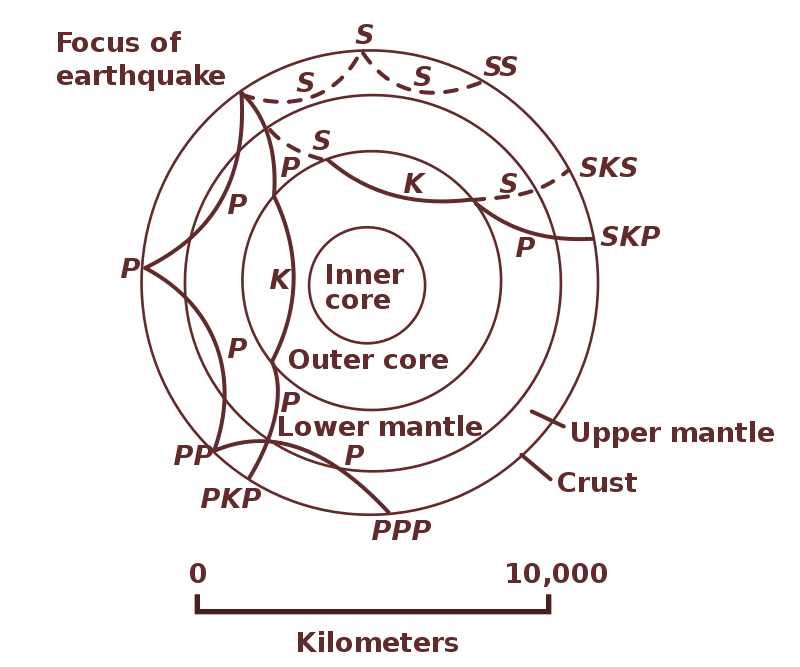
\includegraphics[width=.65\textwidth]{wave_path.png}
            \end{figure}
        \end{column}
        \begin{column}{0.4\textwidth}
            \begin{figure}
                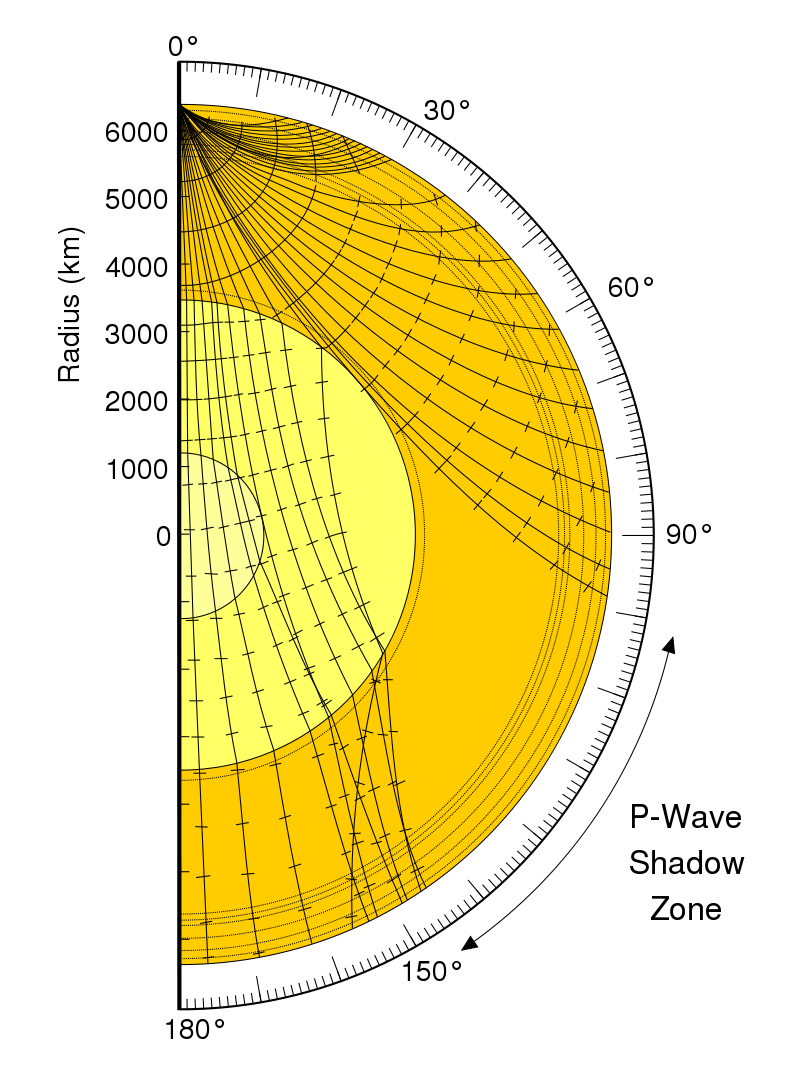
\includegraphics[width=\textwidth]{shadow_zone.png}
            \end{figure}
        \end{column}
    \end{columns}
\end{frame}

\note[itemize]{
\item P-waves (primary) se šíří rychlostí zvuku (poté co vyjdou na vzduch); S-waves (secondary) pomalejší (o cca polovinu) a příčné a pouze v pevných látkách; surface waves jsou pomalejší než oboje dvoje, cestují kolem povrchu Země, dál od povrchu mizí (propagují se na rozhraní dvou médií), dále se dělí na Love waves (L-waves, příčné) a Rayleigh waves (příčné i podélné), při velkých zemětřesení (výbuchu) mohou oběhnout mnohokrát zeměkouli \dots
\item  Surface waves are caused when P waves and S waves come to the surface. 
\item The path that a wave takes between the focus and the observation point is often drawn as a ray diagram. An example of this is shown in a figure above. When reflections are taken into account there are an infinite number of paths that a wave can take. Each path is denoted by a set of letters that describe the trajectory and phase through the Earth. In general an upper case denotes a transmitted wave and a lower case denotes a reflected wave. The two exceptions to this seem to be "g" and "n". \emph{K is P-wave in the outer core, S is S-wave in the mantle etc}
}

\note{
One of the most important examples of infrasonic waves in nature is in earthquakes. Three principal types of earthquake waves exist: the S-wave, a transverse body wave; the P-wave, a longitudinal body wave; and the L-wave, which propagates along the boundary of stratified mediums. L-waves, which are of great importance in earthquake engineering, propagate in a similar way to water waves, at low velocities that are dependent on frequency. S-waves are transverse body waves and thus can only be propagated within solid bodies such as rocks. P-waves are longitudinal waves similar to sound waves; they propagate at the speed of sound and have large ranges.

When P-waves propagating from the epicentre of an earthquake reach the surface of the Earth, they are converted into L-waves, which may then damage surface structures. The great range of P-waves makes them useful in identifying earthquakes from observation points a great distance from the epicentre. In many cases, the most severe shock from an earthquake is preceded by smaller shocks, which can be detected by seismographs and provide advance warning of the greater shock to come. Underground nuclear explosions also produce P-waves, allowing them to be monitored from any point in the world if they are of sufficient intensity.}
\note{The development of extremely sensitive detectors to monitor such explosions has contributed to the maintenance of the Nuclear Test-Ban Treaty, which was signed in 1963 and banned all tests of nuclear weapons except those conducted underground so as to limit the amount of radioactive fallout in the atmosphere.

Infrasonic disturbances of the atmosphere that may extend to 50 km (30 miles) above Earth’s surface are often associated with severe earthquakes. These waves can travel considerable distances around the globe.}

\begin{frame}{Infrazvuk vs seizmické vlny}
    \begin{figure}[h]
        \centering
        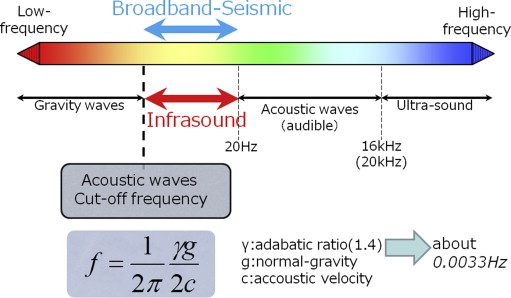
\includegraphics[width=.7\textwidth]{infrasound_vs_seismic.jpg}
    \end{figure}
\end{frame}

\note{
    \textbf{Fig.} Schematic diagram of the characteristics of infrasound waves propagating in the atmosphere. The “infrasound” is defined as sub-audible sounds, as the pressure waves with frequencies ranging from cut-off frequency of sound (3.21 mHz, for a 15 °C isothermal atmosphere) to the lowest frequency of human audible band (20 Hz). Infrasound waves propagate more than few 1000 km along the Earth's surface.
}

\begin{frame}{Monitorování erupcí sopek}
    \begin{columns}
        \begin{column}{.5\textwidth}
            \begin{figure}[h]
                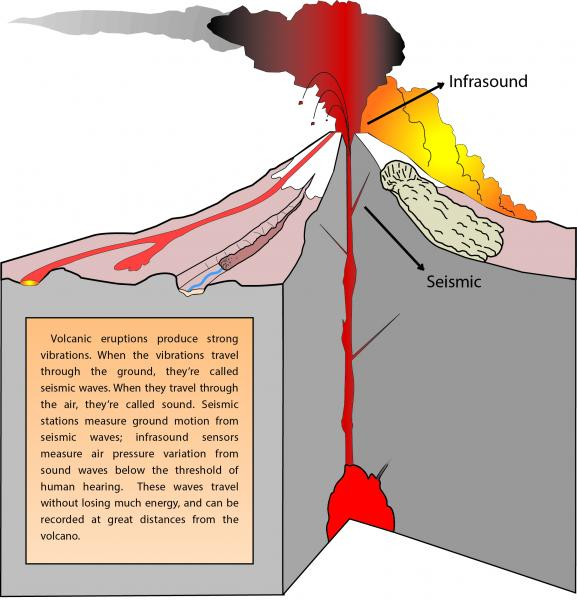
\includegraphics[height=.6\textheight]{volcano.jpg}
                \caption{\cite{volcano2}}
            \end{figure}
        \end{column}
        \begin{column}{.5\textwidth}
            \begin{figure}[h]
                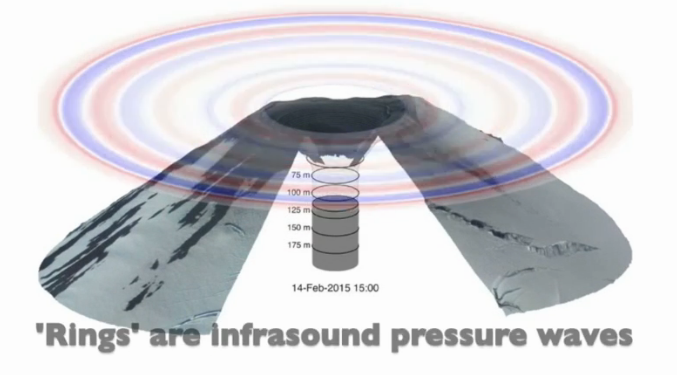
\includegraphics[height=.4\textheight]{volcano.png}
            \end{figure}
        \end{column}
    \end{columns}
\end{frame}

\note[itemize]{
\item "What's nice about infrasound is that we are able to gather information farther from the source than with traditional ground-based monitoring methods," Matoza explained. "Typically, seismic signals from eruptions don't propagate more than a few hundred kilometers from the source. With Calbuco, for example, you can see the eruption very clearly on the local monitoring stations and out to about 250 kilometers on regional seismic networks, but with infrasound, the signal propagates \textbf{in the atmosphere for more than 5 000 kilometers}. What's more, infrasound delivers different information than seismic data alone."
\item nejlepší je vždy kombinovat několik metod
}

\note[itemize]{\scriptsize
\item Infrasound waves travel at the speed of sound, approximately 340 m/s (760 mph) at sea level, thus taking about 15 minutes to travel every 300 km (185 miles). The propagation velocity of infrasound waves is about 10 times slower than seismic waves. This velocity is determined by the temperature and wind structure in the atmosphere, and therefore a detailed knowledge of the atmosphere and the prevailing winds is necessary to understand the long-range propagation of sound. Other sources of infrasound include wind, surf, meteors, glaciers, thunder, and aircraft. Because there are many causes of infrasound, information is needed about the direction, amplitude, duration, and frequency content of infrasound waves to determine what specifically generated the signal. 
\item Monitoring volcanic eruptions in Alaska is challenging due to the remoteness of many of the volcanoes, making a local monitoring network (e.g. seismic) difficult to establish and maintain. Cloudy weather and delays in satellite image acquisition limit how quickly satellites may detect eruptions. Because infrasound is not affected by cloud-cover and can travel long distances, it is a useful tool to detect and monitor volcanic eruptions in Alaska and other locations worldwide. When a volcano produces infrasound, it provides clear evidence that the volcanic vent is open to the atmosphere. Volcanic seismicity is attributed primarily to fracturing rock and fluid movement beneath the surface, so combining infrasound and seismic data helps determine whether a volcano is erupting or whether the activity is confined below the surface. 
}

\begin{frame}{Monitorování erupcí sopek na Aljašce}
    \begin{figure}[h]
        \centering
        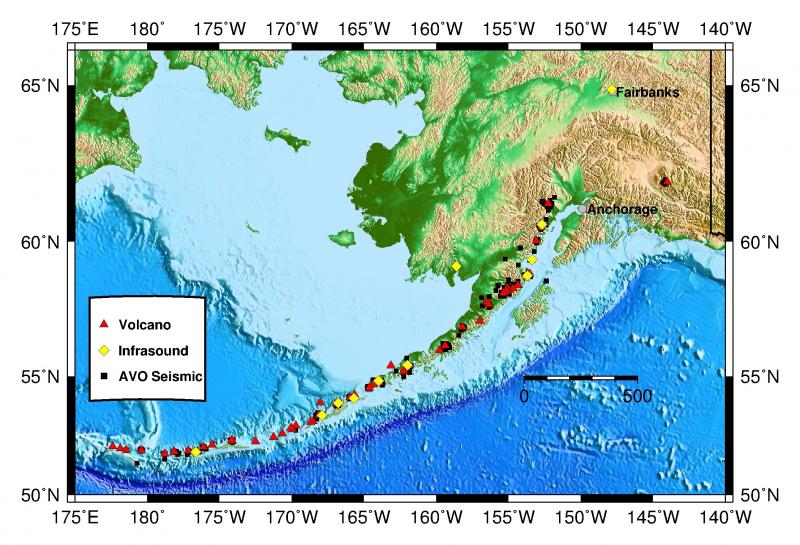
\includegraphics[width=\textwidth]{volcano_monitoring.jpg}
        \caption{\cite{volcano2}}
    \end{figure}
\end{frame}

\begin{frame}{Počasí}
    \begin{itemize}
        \item Monitorování stratosféry pomocí infrazvuku -> potenciálně lepší předpovědi počasí \cite{stratosfera}
        \item Předpovídání tornád \cite{tornado2}
            \begin{figure}[h]
                \centering
                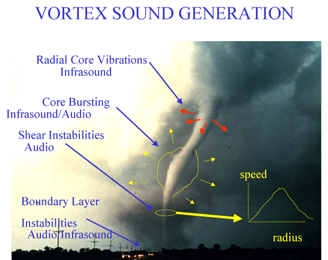
\includegraphics[width=.45\textwidth]{tornado.png}
            \end{figure}
    \end{itemize}
\end{frame}

\note[itemize]{
\item monitorování stratosféry i předpovídání tornád jsou nové nápady (z roku 2018)
\item \textbf{Tornáda} Infrazvuk z bouří, ze kterých se vytvoří tornáda, může být emitován o více než hodinu dříve než dojde k vytvoření tornáda; tato metoda může zlepšit varovný systém proti tornádům; “By monitoring tornadoes from hundreds of miles away, we’ll be able to decrease false alarm rates and possibly even increase warning times,” Elbing said. “It also means storm chasers won’t need to get so close.”
\item \textbf{Tornado formation} No two tornadoes are the same, but all tornadoes require on specific conditions to form. It starts when sunshine heats the ground, which causes pockets of air to rise. If the atmosphere is unstable, the pockets can rise to great heights, resulting in the development of much deep, strong currents of ascending air (updraughts) and storm clouds. If the atmospheric winds are strong enough, the stormy updraughts can start to rotate, and tilt to become vertical. Eventually, the rotation may become so strong that a narrow column of violently rotating air forms — thus, a tornado is born.
}

\note[itemize]{
\item \textbf{Tornáda 2} To listen to infrasound in the atmosphere, the researchers use three infrasound microphones at Oklahoma State University arranged in a triangle, each spaced about 200 feet apart.
\item Two key differences distinguish these microphones from the kind we are used to seeing. "First, these are larger for greater sensitivity to lower frequencies," Elbing said. "Second, we need to get rid of wind noise. ... We seal the microphone inside a container with four openings. A soaker hose—just like the ones used in gardens—is attached to each of these openings and stretched out in opposite directions."

Elbing and his team then parse out the tornado infrasound from the wind noise. "Wind noise is incoherent, so if you average it over a large space it will sum up to zero," he said. "Conversely, tornado infrasound is coherent—meaning waves look alike—over large distances, so the pressure waves add together and contain information."
}

\note{
    \textbf{Stratosfera} This is of particular importance during a particular weather phenomenon, the sudden stratospheric warming (SSW), explains Smets. In mid-February such an event was responsible for the coldest week of this winter in the Netherlands. "Such a sudden warming of the stratosphere is an important characteristic of the winter atmosphere in the northern hemisphere. During this short-lived phenomenon the stratosphere exerts a strong influence on the layer beneath it, the troposphere. This has consequences for the weather and for weather forecasts. In recent years attempts have been made to improve predicting the stratospheric variability using numerical weather forecasts. However, this requires extra independent observations of the upper atmosphere, and this is an area that is extremely difficult to observe. Wind observations, for example, are lacking in weather models past the middle of the stratosphere, higher than around 30 km."

Read more at: \url{https://phys.org/news/2018-03-inaudible-infrasound-weather-climate.html}
}

\begin{frame}{Detekce infrazvuku}
    \begin{itemize}
        \item Mikrofony (normální měřící mikrofony mají cut-off na 3 Hz)
        \item Infrazvukové senzory (mikrobarometry)
            \begin{itemize}
                \item Absolutní a relativní
                    $$p_{total}=p_{static}+p_{sound},$$\ \cite{wiki4}  
            \item Rozmístění více senzorů pohromadě, tzv. ``arrays''
                \item např. Comprehensive Nuclear-Test-Ban Treaty Organisation (CTBTO)
            \end{itemize}
        \item \textbf{Problém} pozadí (vítr, doprava, v podstatě cokoliv)
        \item Balóny ve stratosféře
    \end{itemize}
\end{frame}

\note[itemize]{
\item Comprehensive Nuclear-Test-Ban Treaty (CTBT) -> stanice po celém světě; tam ty detektory nazývají mikrobarometry
\item Multiple types of infrasound sensors exist and are divided into two categories: absolute and differential pressure sensors. \textbf{Absolute} sensors record very small changes in \textbf{background atmospheric pressure}, while \textbf{differential} sensors output small changes in pressure \textbf{relative to a reference pressure}. After the pressure wave is recorded, it is digitized by attached electronics and transmitted to AVO via radio, Internet, or satellite communications (similar to a seismic station). AVO often deploys infrasound microphones in groups, called arrays, and uses the relative arrival times of acoustic waves on each sensor to determine where the sound is coming from 
}

\begin{frame}{Infrasound array}
    \begin{figure}[h]
        \centering
        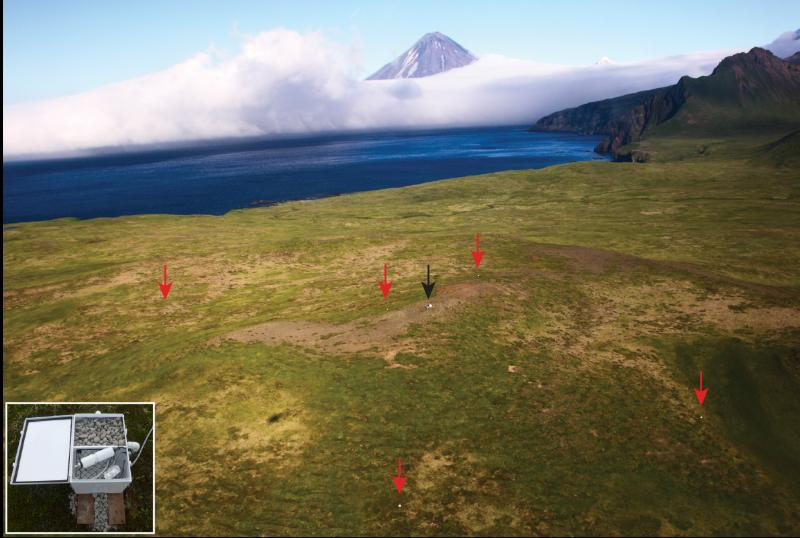
\includegraphics[width=.9\textwidth]{array.jpg}
        \caption{Černě je seismograf, \cite{volcano2}}
    \end{figure}
\end{frame}

\begin{frame}{Infrasound Station IS18, Qaanaaq (Grónsko)}
    \begin{figure}[h]
        \centering
        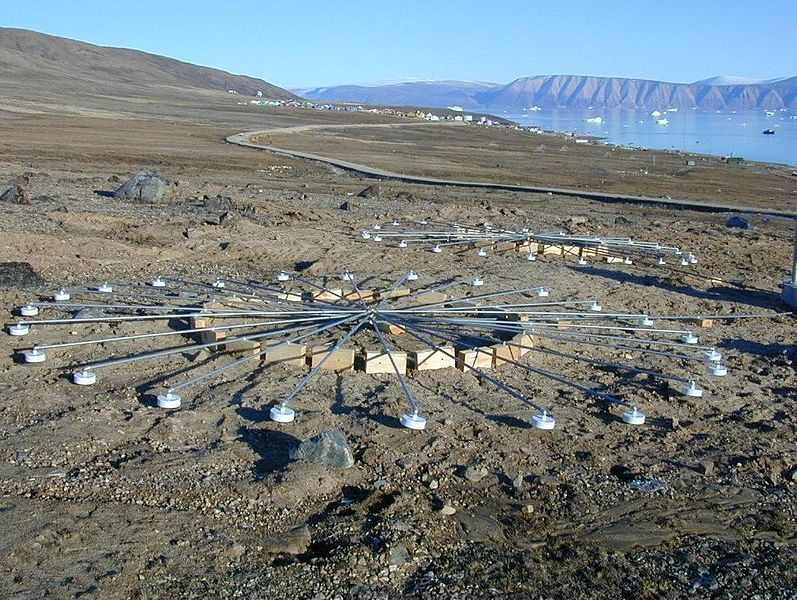
\includegraphics[height=.75\textheight]{array2.jpg}
        \caption{CTBTO, \cite{gronsko}}
    \end{figure}
\end{frame}

\note{
Around the clock, the array monitors the entire world for distinctive blast patterns produced by such explosions, as their unique pattern of ultra-low frequency sound waves persist even when ricocheting through the Earth’s surface.

More broadly, the range of sounds IS18 can detect doesn’t only include mankind’s attempts to annihilate itself. Infrasound is used to trace earthquakes, locate petroleum deposits based on their movements, and monitor the human heart in ballistocardiography. When viewed in this light, it seems like Greenland’s observatory at the end of the world is keeping tabs on the pulse of us all, perhaps on an even more enormously important scale than we thought.
}

\begin{frame}{Infrazvukový vs seizmický signál}   
    \begin{figure}[h]
        \centering
        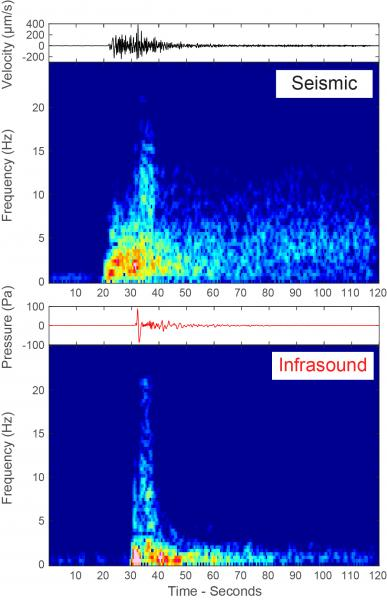
\includegraphics[height=.67\textheight]{signal.jpg}
        \caption{\scriptsize Explosion signals from Cleveland volcano recorded on 21 July 2015 at a station 3.9 km (2.4 miles) from the summit of the volcano. Note the characteristic delay in the arrival of the infrasound signal ~11.5 seconds after the seismic signal. This is due to the lower propagation velocity of sound in the atmosphere than in the Earth. \cite{volcano2}}
    \end{figure}
\end{frame}


% různá nastavení
%\begin{overlayarea}{\textwidth}{\textheight}\end{overlayarea}


\appendix
\begin{frame}[allowframebreaks]{Reference}
    \nocite{*}
\renewcommand*{\bibfont}{\tiny}
\printbibliography
\end{frame}

\end{document}
